% =====================================================================
% Clase -- Geometría 9° -- Trimestre I -- Semana 04
% Sesión 004 (jue 24 sep., 13:00, 40 min)
% Tema: Semejanza de figuras
% Subtema: Criterios de semejanza de triángulos
% Hilo conductor del trimestre I: «Eratóstenes mide la Tierra con una sombra»
% Tema 1 de la guía: Semejanza de figuras (tema:semejanza)
% Material del docente (no se entrega a los estudiantes).
% =====================================================================
\documentclass[11pt]{article}
\makeatletter\def\input@path{{../../../../../plantillas/estilo/}}\makeatother
\usepackage{mmcantillo}
\guiadelestudiante{../../guia-didactica/guia-periodo-I-semejanza-medicion}

\tipodocumento{Clase}
\asignatura{Geometría}
\titulo{Semana 4: la sombra que mide el mundo}
\grado{9°}
\periodo{I}

% DBA: matematicas grado 9 · DBA 6 — Identifica relaciones de congruencia y semejanza entre
% las formas geométricas que configuran el diseño de un objeto. Evidencias de esta sesión:
% «Compara figuras y argumenta la posibilidad de ser congruentes o semejantes entre sí» y
% «Utiliza criterios para argumentar la semejanza de dos triángulos».

\begin{document}

\encabezado*

\begin{center}
{\renewcommand{\arraystretch}{1.3}
\begin{tabularx}{\linewidth}{@{}l l l X l@{}}
  \toprule
  \textbf{Sesión} & \textbf{Fecha} & \textbf{Min} & \textbf{Subtema} & \textbf{Entregables}\\
  \midrule
  004 & jue 24 sep., 13:00 & 40 & Criterios de semejanza de triángulos & Se deja tarea\\
  \bottomrule
\end{tabularx}}
\end{center}

Segundo paso del hilo. La semana pasada vimos qué significa que dos figuras sean semejantes;
hoy aparecen los tres criterios que permiten \emph{demostrarlo} sin medirlo todo. Con uno de
ellos —el más simple— Eratóstenes midió la Tierra sin salir de Egipto.
Referencia: \refguia{tema:semejanza}.

% ---------------------------------------------------------------------
\seccion{Sesión 004 — jueves 24 de septiembre · 13:00 · 40 min}

\textbf{Objetivo.} Reconocer y aplicar los criterios AA, LAL y LLL para justificar que dos
triángulos son semejantes, y usarlos para calcular una longitud inaccesible.

\textbf{Materiales.} Tablero; regla y transportador; la guía.

\begin{center}
{\renewcommand{\arraystretch}{1.3}
\begin{tabularx}{\linewidth}{@{}l l X@{}}
  \toprule
  \textbf{Momento} & \textbf{Min} & \textbf{Actividad}\\
  \midrule
  Enganche & 0--6 & En el patio (o desde la ventana) hay un árbol o un poste. «¿Cómo lo
    medimos sin treparnos ni usar escalera?» Dejar que propongan. Alguien dirá lo de la
    sombra: ese es el camino.\\
  Los tres criterios & 6--20 & \textbf{AA}: dos ángulos iguales bastan (el tercero se
    deduce, porque suman $180^\circ$). \textbf{LAL}: dos lados proporcionales y el ángulo
    comprendido igual. \textbf{LLL}: los tres lados proporcionales. Dibujo de cada uno en
    el tablero, marcando con arcos los ángulos y con rayitas los lados.
    \textbf{Semejante no es congruente}: misma forma, distinto tamaño.\\
  La sombra & 20--32 & Volver al árbol. Los rayos del Sol llegan paralelos, así que el
    poste y el árbol hacen con su sombra dos triángulos rectángulos con el mismo ángulo de
    elevación: son semejantes por AA. Plantear la proporción y resolver con números
    concretos (poste \qty{4}{m}, sombra \qty{6}{m}; sombra del árbol \qty{21}{m}).
    Y aquí el remate del hilo: es exactamente lo que hizo Eratóstenes, pero con la Tierra
    entera.\\
  Cierre & 32--40 & Dejar la tarea y anticipar la sesión 005: si la razón de semejanza es
    $1$, los triángulos son \emph{congruentes} — y ahí los criterios cambian de nombre.\\
  \bottomrule
\end{tabularx}}
\end{center}

\textbf{Figura para el tablero: la misma hora, el mismo ángulo.}

\begin{center}
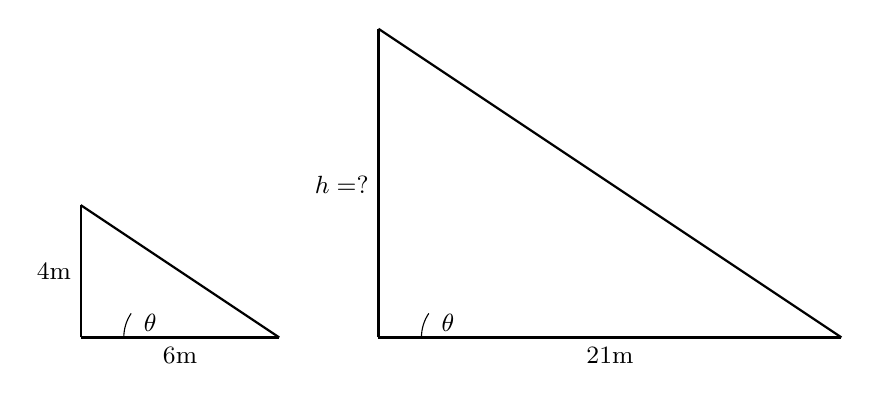
\begin{tikzpicture}[scale=0.42, font=\small]
  % poste
  \draw[thick] (0,0) -- (0,4);
  \draw[thick] (0,0) -- (6,0);
  \draw[thick] (0,4) -- (6,0);
  \draw (1.3,0) arc (180:146:1.3);
  \node at (2.1,0.45) {$\theta$};
  \node[left] at (0,2) {\qty{4}{m}};
  \node[below] at (3,0) {\qty{6}{m}};
  % arbol
  \begin{scope}[xshift=9cm]
    \draw[thick] (0,0) -- (0,14/1.5);
    \draw[thick] (0,0) -- (21/1.5,0);
    \draw[thick] (0,14/1.5) -- (21/1.5,0);
    \draw (1.3,0) arc (180:146:1.3);
    \node at (2.1,0.45) {$\theta$};
    \node[left] at (0,4.6) {$h = ?$};
    \node[below] at (7,0) {\qty{21}{m}};
  \end{scope}
\end{tikzpicture}

{\small Mismo ángulo de elevación del Sol $\Rightarrow$ triángulos semejantes por AA
$\Rightarrow$ $\dfrac{h}{21} = \dfrac{4}{6}$.}
\end{center}

\begin{nota}
\textbf{El error que hay que cazar.} «Tres ángulos iguales $\Rightarrow$ congruentes» es falso
y aparece impreso en el módulo de Geometría de \texttt{recursos/} (lo trae como primer criterio
de congruencia). Da \emph{semejanza}. El contraejemplo es de un segundo: $3$-$4$-$5$ y
$6$-$8$-$10$. Si algún estudiante lo trae de un libro o de internet, es buena ocasión para
mostrarlo.
\end{nota}

\begin{nota}
\textbf{40 minutos alcanzan justo.} Si el enganche se alarga, el ejemplo numérico de la sombra
se puede pasar a la tarea (es su pregunta 3) y usar los minutos en los tres criterios, que es
lo que no puede quedar a medias.
\end{nota}

\begin{nota}
Los cuatro ejercicios de la tarea son nuevos en el banco
(\texttt{recursos/banco/matematicas/semejanza-triangulos-9.py}): solo había semejanza de 5°
(escalas y rectángulos), nada sobre los criterios en triángulos.
\end{nota}

\end{document}
